%!TEX root = pfc-memoria.tex
%!TEX encoding = UTF-8 Unicode

\chapter{Manual de instalación}

\epigraph{``Tenemos que dejar de optimizar para programadores y comenzar a optimizar para usuarios.''}{\textsc{Jeff Atwood}}

En este capítulo se describe el procedimiento de instalación de la aplicación y las bibliotecas de las que depende.

\section{Instalación de prerrequisitos}



\chapter{Manual de usuario}

\epigraph{``Los ordenadores son buenos siguiendo instrucciones, no leyendo tu mente.''}{\textsc{Donald Knuth} (1938--)}

\section{Carga del fichero de entrenamiento}

La primera pantalla que se muestra al abrir la aplicación es la pestaña de carga (\autoref{fig:ss-01-load-tab}).

\begin{figure}[H]
\centering
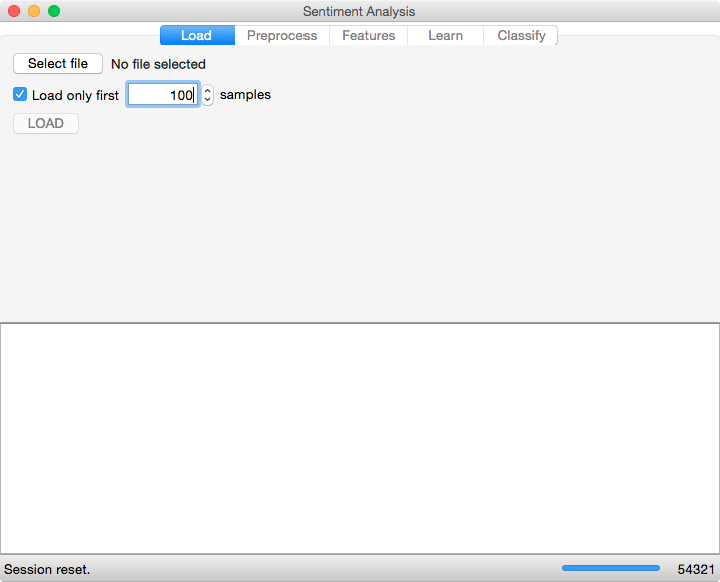
\includegraphics[width=13cm]{ss-01-load-tab}
\caption{Pantalla de carga del fichero de entrenamiento}
\label{fig:ss-01-load-tab}
\end{figure}

\newpage
Al pulsar sobre el botón \menu{Select file} aparece un cuadro de diálogo que permite seleccionar el fichero \path{train.tsv} de entrenamiento (\autoref{fig:ss-02-load-file}).

\begin{figure}[H]
\centering
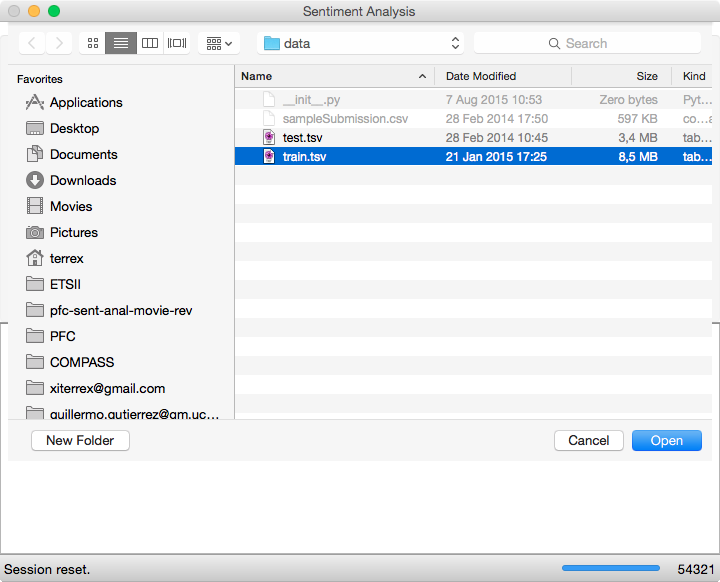
\includegraphics[width=14cm]{ss-02-load-file}
\caption{Pantalla de selección del fichero de entrenamiento}
\label{fig:ss-02-load-file}
\end{figure}

\newpage
Una vez seleccionado, marcar la opción de carga parcial si se desea, indicando el número de muestras. A continuación, pulsar el botón \menu{LOAD}, con lo que aparece el fichero en forma de tabla en el panel de datos (\autoref{fig:ss-03-file-loaded}).

\begin{figure}[H]
\centering
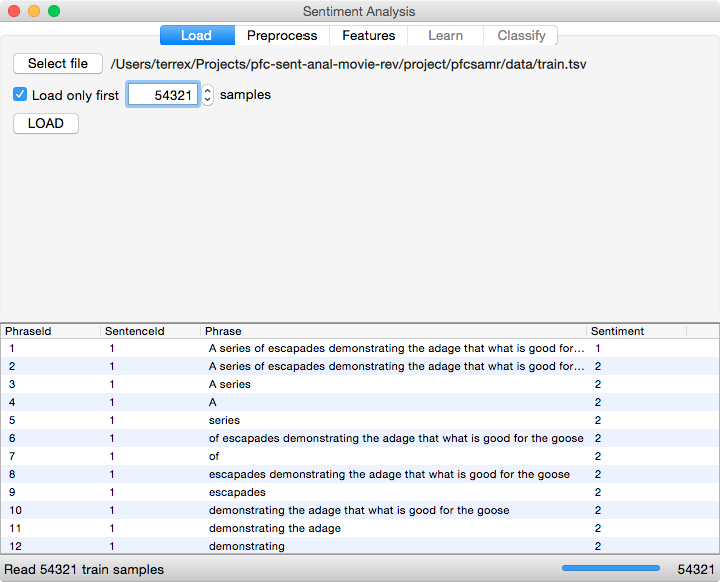
\includegraphics[width=14cm]{ss-03-file-loaded}
\caption{Pantalla con el fichero de entrenamiento cargado}
\label{fig:ss-03-file-loaded}
\end{figure}

\newpage
\section{Opciones de preprocesamiento de texto}
\label{sec:manual-preproc}

Una vez cargado, pasamos a la siguiente pestaña de opciones de preprocesamiento. En esta pantalla, marcamos las opciones deseadas, y a continuación pulsamos el botón \menu{RUN} para proceder al preprocesamiento. Se muestra una barra de progreso a la derecha de la barra de estado, y al terminar, se actualiza el panel de datos con las muestras preprocesadas (\autoref{fig:ss-04-preproc-tab}).

\begin{figure}[H]
\centering
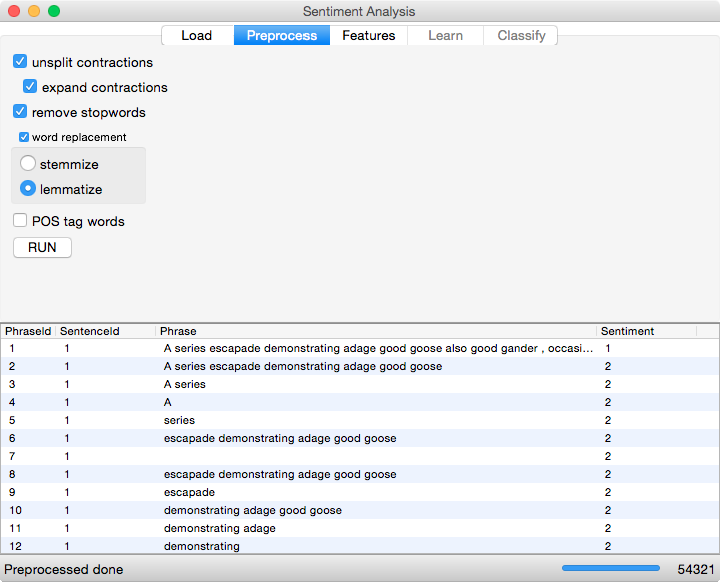
\includegraphics[width=14cm]{ss-04-preproc-tab}
\caption{Pantalla de opciones de preprocesamiento}
\label{fig:ss-04-preproc-tab}
\end{figure}

\newpage
\section{Extracción de características}
\label{sec:manual-features}

El siguiente paso es la extracción de características. Pulsar en la pestaña y marcar las opciones deseadas para la extracción de n-gramas y su reducción. Pulsar en el botón \menu{RUN} para proceder con la transformación. Al finalizar, se muestra el panel de datos con una característica en cada columna, y su valor para cada muestra. El encabezado de la columna indica el n-grama concreto (\autoref{fig:ss-05-feat-tab}).

\begin{figure}[H]
\centering
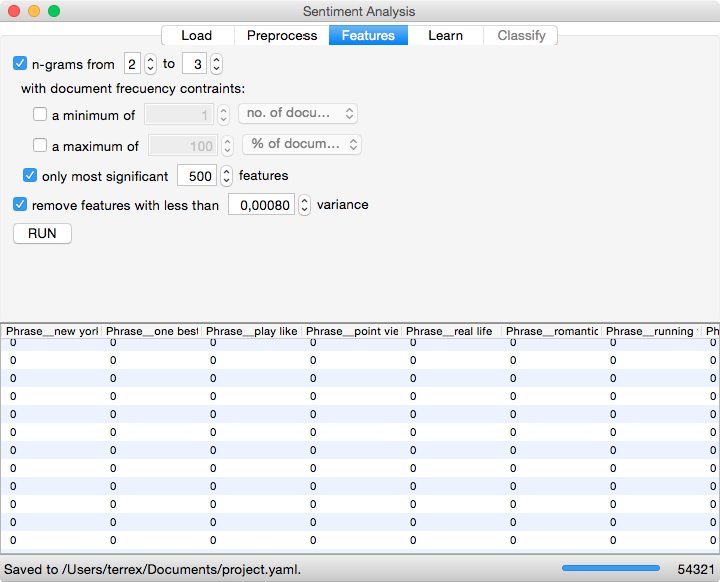
\includegraphics[width=14cm]{ss-05-feat-tab}
\caption{Pantalla de opciones de extracción de características}
\label{fig:ss-05-feat-tab}
\end{figure}

\newpage
\section{Aprendizaje automático del modelo}
\label{sec:manual-learn}

A continuación, avanzamos de pestaña para las opciones de aprendizaje. Se recomienda dejar marcado la división del conjunto en subconjunto de entrenamiento y subconjunto de autoevaluación, para poder obtener una puntuación del modelo aprendido.

Elegir el modelo concreto en la segunda fila de pestañas y pulsar el botón \menu{RUN}. Cuando finalice el aprendizaje, se actualizará el valor de la puntuación (etiqueta \codet{SCORE: }). Hay cinco modelos a elegir, no es obligatorio entrenarlos todos, pero está bien hacerlo para comparar su puntuación y elegir el mejor.

Se puede repetir tantas veces como se desee e ir alterando los parámetros para encontrar la mayor puntuación (\autoref{fig:ss-06-learn-tab}).

\begin{figure}[H]
\centering
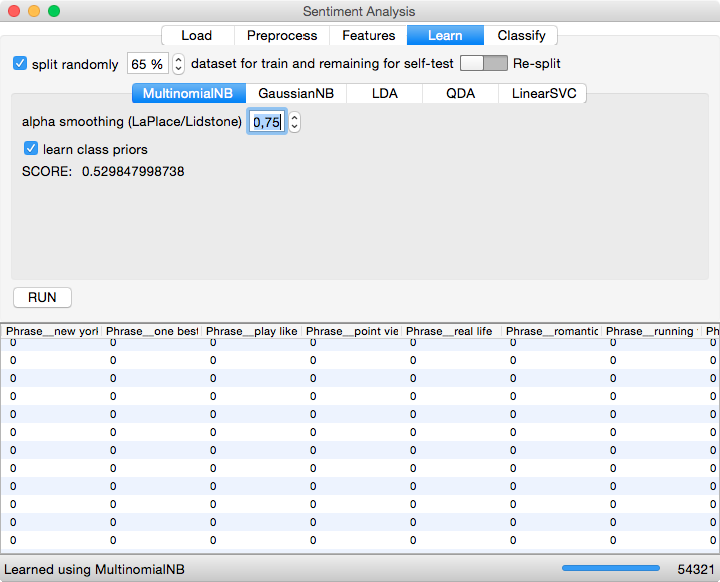
\includegraphics[width=14cm]{ss-06-learn-tab}
\caption{Pantalla de aprendizaje (\codep{MultinomialNB})}
\label{fig:ss-06-learn-tab}
\end{figure}

\newpage
\section{Clasificación del conjunto de clasificación}

Una vez entrenado alguno de los modelos, avanzar pulsando la pestaña siguiente (\autoref{fig:ss-07-classify-tab}). Pulsar el botón \menu{Select file} para elegir el fichero \path{test.tsv} de evaluación.

\begin{figure}[H]
\centering
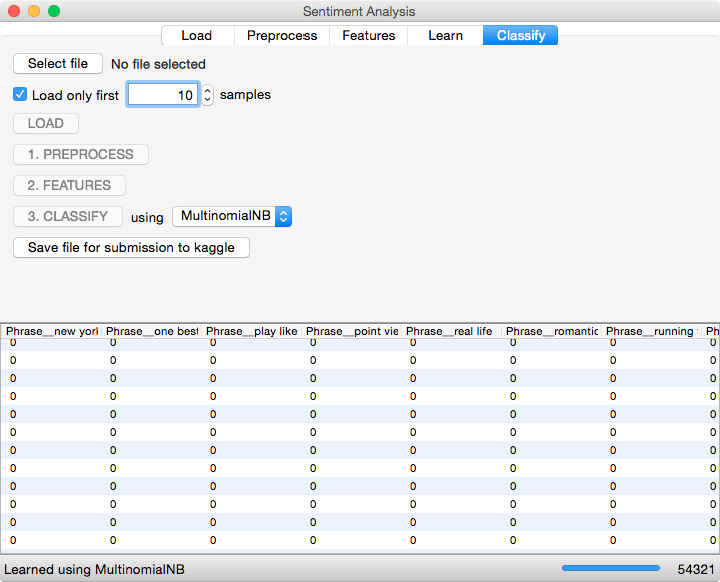
\includegraphics[width=14cm]{ss-07-classify-tab}
\caption{Pantalla de la pestaña de clasificación}
\label{fig:ss-07-classify-tab}
\end{figure}

\newpage
Se puede activar la opción de carga parcial e indicar el número de muestras, si se desea. A continuación pulsar \menu{LOAD} para realizar la carga y la visualización en el panel de datos (\autoref{fig:ss-08-classify-test-loaded}).

\begin{figure}[H]
\centering
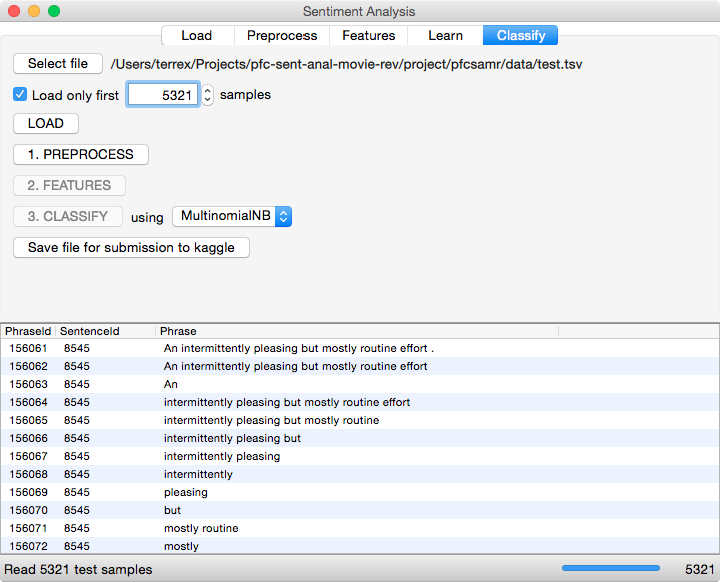
\includegraphics[width=14cm]{ss-08-classify-test-loaded}
\caption{Pantalla con el conjunto de clasificación cargado}
\label{fig:ss-08-classify-test-loaded}
\end{figure}

\newpage
Pulsando el botón \menu{1. PREPROCESS} se realiza el preprocesamiento de texto de clasificación de manera análoga a como se preprocesó el texto de entrenamiento en la fase de entrenamiento (\autoref{sec:manual-preproc}). Se actualizará el panel de datos con el resultado (\autoref{fig:ss-08-classify-test-loaded}).

\begin{figure}[H]
\centering
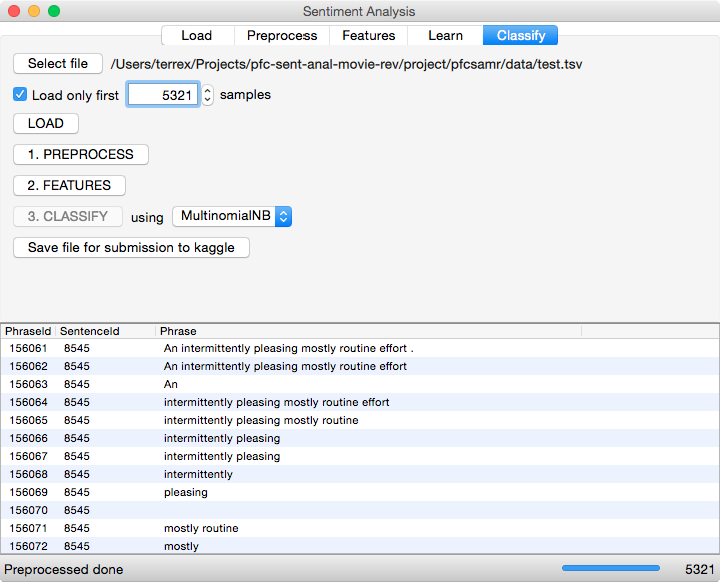
\includegraphics[width=14cm]{ss-09-classify-test-preproccesed}
\caption{Pantalla con el texto preprocesado}
\label{fig:ss-09-classify-test-preproccesed}
\end{figure}

\newpage
Siguiendo con el procedimiento, pulsamos el botón \menu{2. FEATURES} para extraer las características del texto de clasificación preprocesado, que se realiza automáticamente de manera análoga a como se hizo en la fase de entrenamiento (\autoref{sec:manual-features}). Al terminar, se muestra en el panel de datos las características de las muestras a clasificar (\autoref{fig:ss-10-classify-test-featured}).

\begin{figure}[H]
\centering
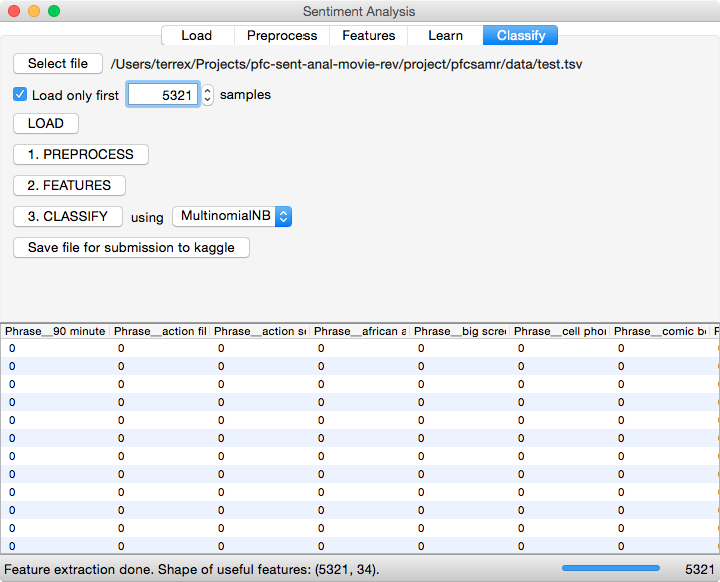
\includegraphics[width=14cm]{ss-10-classify-test-featured}
\caption{Pantalla de características}
\label{fig:ss-10-classify-test-featured}
\end{figure}


\newpage
El último paso es realizar las predicciones. Para ello, elija un modelo del cuadro desplegable. Este modelo debería haber sido entrenado previamente en el paso de entrenamiento (\autoref{sec:manual-learn}), en caso contrario se mostrará un error. Pulsar el botón \menu{3. CLASSIFY} para clasificar las muestras. Aparecerá en el panel de datos las muestras originales con una columna añadida del sentimiento predicho por el modelo seleccionado (\autoref{fig:ss-11-classify-test-predictions}). Si se desea, se puede repetir usando otro modelo.

\begin{figure}[H]
\centering
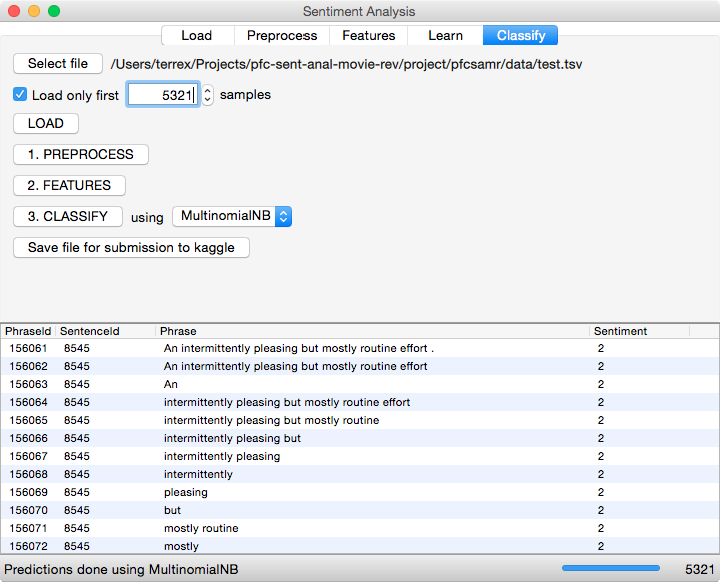
\includegraphics[width=14cm]{ss-11-classify-test-predictions}
\caption{Pantalla con las predicciones de sentimiento}
\label{fig:ss-11-classify-test-predictions}
\end{figure}

Posteriormente, pulsando el botón \menu{Save file for submission to kaggle} se puede guardar el resultado de la clasificación en el formato \path{.csv} para posteriormente entregar en Kaggle.\footnote{\url{https://www.kaggle.com/c/sentiment-analysis-on-movie-reviews}}

\newpage
En cualquier momento, se puede usar el menú \menu{File} para reiniciar el sistema, o abrir o guardar las opciones de la sesión para reanudar posteriormente.

\begin{figure}[H]
\centering
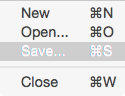
\includegraphics[width=\textwidth]{ss-12-menu-file}
\caption[Pantalla con el menú \codet{FILE}]{Pantalla con el menú \menu{File}}
\label{fig:ss-12-menu-file}
\end{figure}

